\section{Zahlen und Zahlenmengen}

\subsection{Natürliche Zahlen}

Die Zahlen $1,2,3,4,5,\ldots$, die man beim Abzählen irgendwelcher Gegenstände verwendet, bezeichnet man als \textbf{natürliche Zahlen}. Die Folge der natürlichen Zahlen endet nie. Nach Cantor stellt die Menge $\mathbb{N}$ der natürlichen Zahlen eine sogenannte »abzählbar unendliche Menge« dar.

Was \emph{ist} eine Zahl, beispielsweise die Zahl 3? Man kann sich die 3 als die abstrakte Eigenschaft denken, die z.\,B. 3 Äpfel, 3 Autos und 3 Träume gemeinsam haben. Darüber hinausgehende Fragen zum \emph{Wesen} der Zahlen gehören eher in den Grenzbereich von Mathematik und Philosophie. Die Mathematik sieht es als ihre Hauptaufgabe, formale strukturmäßige Zusammenhänge zwischen den von ihr betrachteten Objekten zu untersuchen -- dazu gehört das \textbf{Rechnen}, mit dem wir uns im nächsten Kapitel befassen.

\subsection{Ganze Zahlen}

Gleichungen der Form $a + x = b$ mit gegebenen natürlichen Zahlen $a$ und $b$ lassen sich in $\mathbb{N}$ offenbar nicht uneingeschränkt lösen: Sobald $a \geq b$ ist, hat die Gleichung $a + x = b$ keine Lösung für $x$ in $\mathbb{N}$. Ein Beispiel ist die Gleichung $10 + x = 7$, für die man keine natürliche Zahl für $x$ finden wird, damit die Gleichung stimmt. (Mit dem Lösen von Gleichungen werden wir uns an späterer Stelle ausführlich beschäftigen.)

Die Lösbarkeit kann dadurch erreicht werden, indem die Menge $\mathbb{N}$ durch Hinzunahme der Null und der negativen, ganzen Zahlen $-1, -2, -3, -4, -5, \ldots$ zur Menge $\mathbb{Z}$ aller \textbf{ganzen Zahlen} erweitert wird. Die obige Gleichung $10 + x = 7$ hat nun die Lösung $x = -3$.

Die ganzen Zahlen in $\mathbb{Z}$ können durch Punkte auf der sogenannten \textbf{Zahlengeraden} veranschaulicht werden. Die Zahlengerade ist eine Gerade mit willkürlich gewähltem Nullpunkt und Einheitspunkt 1. Die positiven Zahlen werden vom Nullpunkt aus nach rechts und die negativen Zahlen vom Nullpunkt aus nach links abgetragen.

\begin{center}
  \begin{tikzpicture}[x=1cm]
    \draw[-{Stealth}] (-4.2,0) -- (4.4,0);
    \foreach \x in {-3,...,3} {
      \draw (\x,-0.12) -- (\x,0.12);
      \node[below=2pt] at (\x,0) {\x};
    }
    \node at (-4.0,0.5) {$\ldots$};
    \node at (4.2,0.5) {$\ldots$};
  \end{tikzpicture}
\end{center}

Bevor wir über weitere Zahlenbereiche wie Brüche usw. reden, ist es zur Vorbereitung sinnvoll, in einem kurzen Abschnitt die Verwendung von Variablen zu behandeln.

\subsection{Die Verwendung von Variablen}

Im vorigen Abschnitt über die ganzen Zahlen haben wir bereits eine Gleichung hingeschrieben:
\[ a + x = b \]

Solche und ähnliche Gleichungen werden uns noch häufig beschäftigen. An dieser Stelle wollen wir zunächst nur auf die Frage hinaus, was die Buchstaben $a$, $b$ und $x$ bedeuten.

Eigentlich müssten sich die Leser aus der Schulzeit (wenn auch vielleicht ungern) an die Verwendung von \textbf{Variablen} als Platzhalter für Zahlen erinnern. Sie werden beispielsweise verwendet, um gewisse allgemein gültige Sachverhalte in knapper Form auszudrücken. Wenn ich etwa sage:
\begin{quote}
  »Für jede Zahl $x$ gilt $x + 3 = 3 + x$«,
\end{quote}
so habe ich damit eine allgemeine Wahrheit knapp beschrieben, denn ich weiß nun, dass ich für $x$ jeden Wert einsetzen kann (z.\,B. $x = 5$, $x = -8{,}2$ oder $x = 1\,000\,000$), und immer stimmt die Aussage.

Beim Thema Gleichungen ist es meist so, dass eine Variable nicht für \emph{jede}, sondern für \emph{eine bestimmte}, aber im Augenblick noch nicht ausgerechnete Zahl steht. Zum Beispiel stimmt die Gleichung
\[ 5 + x = 7 , \]
wie man leicht sehen kann, nur für den Fall $x = 2$, das man konsequenterweise die \textbf{Lösung} dieser Gleichung nennt.

Wie man sieht, kann es also unterschiedliche Gründe geben, Variablen in mathematischen Ausdrücken zu verwenden. Manchmal deutet man durch die Wahl der unterschiedlichen Buchstaben auch die unterschiedlichen Rollen der Variablen an. Schauen wir noch einmal auf die obige Gleichung
\[ a + x = b . \]
Wenn man hier von einer »Gleichung mit gegebenen $a$ und $b$« spricht, so meint man damit, dass man von festen Zahlen $a$ und $b$ ausgeht (deren genaue Werte einem aber egal sind) und die Lösung für $x$ sucht. $a$ und $b$ werden mitunter als \textbf{Koeffizienten} oder \textbf{Parameter} bezeichnet.

Eine interessante mathematische Aussage lautet dann beispielsweise:
\begin{itemize}
  \item Eine solche Gleichung hat immer die Lösung $x = b - a$.
\end{itemize}

\subsection{Rationale Zahlen}

Jetzt geht es mit den Zahlen weiter.

Den Quotienten $\dfrac{p}{q}$ mit $q \neq 0$ zweier beliebiger, positiver oder negativer, ganzer Zahlen $p$ und $q$ bezeichnet man als \textbf{Bruch}. Es sind die Brüche von allen ganzen Zahlen definiert mit Ausnahme der Division durch die Zahl Null. Beispiele sind $\dfrac{3}{4}$, $\dfrac{-2}{5}$ oder $\dfrac{-2}{-5}$. (Dass die beiden letzten Brüche identisch sind, folgt aus den Rechenregeln des nächsten Kapitels.)

Bei der Darstellung der ganzen Zahlen als Bruch besitzt der Nenner speziell den Wert $q = 1$, mit anderen Worten können die ganzen Zahlen auch als spezielle Brüche (nämlich mit Nenner 1) aufgefasst werden, z.\,B. $5$ als $\dfrac{5}{1}$.

Für die Interpretation des Rechnens mit Brüchen ist wichtig zu wissen, dass die Multiplikation dem »Bruchteil von« entspricht: Zum Beispiel wird »$\tfrac{3}{4}$ von 7« berechnet als $\tfrac{3}{4} \cdot 7$.

Die Zahlenmenge $\mathbb{Q}$, die sich aus den ganzen Zahlen und den (»echten«) Brüchen zusammensetzt, wird als Menge der \textbf{rationalen Zahlen} bezeichnet. Gleichungen der Form $a \cdot x = b$ mit gegebenen $a, b \in \mathbb{Z}$ und $a \neq 0$ sind innerhalb der Menge $\mathbb{Q}$ der rationalen Zahlen uneingeschränkt lösbar.

Bei der \textbf{geometrischen Darstellung} ordnet man jeder rationalen Zahl $\dfrac{p}{q}$ einen Punkt auf einer Zahlengeraden zu. Für $q > 0$ ist dies der Endpunkt der vom Nullpunkt aus nach rechts (für $q < 0$ nach links) abgetragenen Strecke der Länge $\left|\dfrac{p}{q}\right|$.\footnote{Mit $|a|$ ist der \textbf{Betrag} der reellen Zahl $a$ gemeint -- dazu mehr in Abschnitt 1.3.5.}

\begin{center}
  \begin{tikzpicture}[x=1.4cm]
    \draw[-{Stealth}] (-3.2,0) -- (3.4,0);
    \draw (-2,-0.5) -- (-2,0.9);
    \draw (0,-0.5) -- (0,0.9);
    \draw (2,-0.5) -- (2,0.9);
    \draw[<->] (-2,0.5) -- (0,0.5);
    \draw[<->] (0,0.5) -- (2,0.5);
    \node[above] at (-1,0.5) {$\left|\tfrac{p}{q}\right|$};
    \node[above] at (1,0.5) {$\left|\tfrac{p}{q}\right|$};
    \node[below] at (-2,-0.5) {$-\tfrac{p}{q}$};
    \node[below] at (0,-0.5) {$0$};
    \node[below] at (2,-0.5) {$+\tfrac{p}{q}$};
  \end{tikzpicture}
\end{center}

Wenn man sich auf der Zahlengeraden alle Brüche vorstellt, so ist bemerkenswert, dass zwischen irgend zwei Punkten stets noch ein weiterer und damit -- wenn man immer wieder Zwischenpunkte betrachtet -- bereits unendlich viele Punkte liegen. Wird nämlich der rationalen Zahl $\dfrac{p_1}{q_1}$ der Punkt $P_1$ und $\dfrac{p_2}{q_2}$ der Punkt $P_2$ zugeordnet, so liegt beispielsweise der dem arithmetischen Mittel
\[ \frac{1}{2}\left(\frac{p_1}{q_1} + \frac{p_2}{q_2}\right) \]
zugeordnete Punkt $P_3$ sicher zwischen $P_1$ und $P_2$. Die Mathematiker drücken das so aus: Die Brüche liegen »dicht« auf der Zahlengeraden.

\subsection{Reelle Zahlen}

Es könnte angenommen werden, dass mit den rationalen Zahlen die Menge aller Zahlen gefunden ist, die es überhaupt »gibt«. Das ist aber nicht richtig. Es gibt Zahlen, die nicht zu den rationalen Zahlen gehören -- dies sind die \textbf{irrationalen Zahlen}. Jede Zahl, die nicht durch einen Bruch der Form $\dfrac{p}{q}$ (mit ganzen Zahlen $p$ und $q$) dargestellt werden kann, ist eine irrationale oder nicht-rationale Zahl. Dabei unterscheidet man zwischen \textbf{algebraischen Irrationalzahlen} (sie lassen sich in geschlossener Form durch Wurzelausdrücke bzw. als Lösung einer algebraischen Gleichung darstellen, dazu später mehr) und \textbf{nicht-algebraischen, transzendenten Irrationalzahlen}.

\subsubsection{Beispiele}

Algebraisch irrational sind $\sqrt{2}$, $2+\sqrt{3}$, $\sqrt[5]{11}$.

Transzendent irrational sind $e$, $\ln 5$, $\sin 1$.\beispielende

$e$ ist dabei die \textbf{Eulersche Zahl}, der Zahlenwert beträgt $2{,}71828\ldots$ Der Beweis, dass $\sqrt{2}$ kein Bruch ist (also $\sqrt{2} \notin \mathbb{Q}$), ist eines der ältesten und prominentesten Beispiele für einen indirekten Beweis (Widerspruchsbeweis).

Die Gesamtheit aller rationalen und irrationalen Zahlen bildet die Menge $\mathbb{R}$ der \textbf{reellen Zahlen}. Die reellen Zahlen können mit Hilfe der Zahlengeraden geometrisch als Punkte dargestellt werden. Obwohl bereits die den rationalen Zahlen zugeordneten Punkte »dicht« liegen (wir sprachen oben darüber), besitzt die Zahlengerade noch Lücken. Diese werden von sämtlichen Irrationalzahlen ausgefüllt. Die allen reellen Zahlen zugeordneten Punkte füllen die Zahlengerade lückenlos. Man sagt auch, die Menge $\mathbb{R}$ bilde ein \textbf{Kontinuum}.

Die Darstellung auf der Zahlengeraden bildet auch die Grundlage für die auf den reellen Zahlen erklärte \textbf{Ordnung}: Für verschiedene reelle Zahlen $a$ und $b$ ist stets entweder $a < b$ oder $a > b$ ($a$ liegt »links« oder »rechts« von $b$).

Die reellen Zahlen lassen sich, wie aus der Schule bekannt, auch als \textbf{Dezimalzahlen} mit Vor- und Nachkommastellen darstellen. Beispielsweise wird der Bruch $\tfrac{1}{2}$ durch die Dezimalzahl $0{,}5$ und $\tfrac{12}{5}$ durch $2{,}4$ beschrieben. Bei irrationalen Zahlen (die also keine Brüche sind) fällt es schwer, irgendeine andere als die Dezimaldarstellung anzugeben. Wie bereits erwähnt, ist $\sqrt{2}$ eine irrationale Zahl; ihr numerischer Wert ist $1{,}414\ldots$ Es handelt sich um eine \textbf{unendliche nicht-periodische Dezimalzahl}. Allgemein gilt Folgendes:
\begin{itemize}
  \item Fasst man die reellen Zahlen als alle möglichen Dezimalzahlen auf, so entsprechen die rationalen Zahlen genau denjenigen Dezimalzahlen, die nur endlich viele Stellen hinter dem Komma haben (abgesehen von angehängten Nullen) oder aber unendlich viele Stellen, die sich periodisch wiederholen. Anders gesagt: Die irrationalen Zahlen entsprechen genau den Dezimalzahlen, die hinter dem Komma unendlich viele Stellen ohne ein sich wiederholendes Muster haben.
\end{itemize}

Man kann diese Zusammenhänge formal beweisen, doch wir wollen dies hier selbstverständlich nicht tun.

Im folgenden Bild sind die Beziehungen zwischen den bisher behandelten Zahlen noch einmal dargestellt:

\begin{center}
  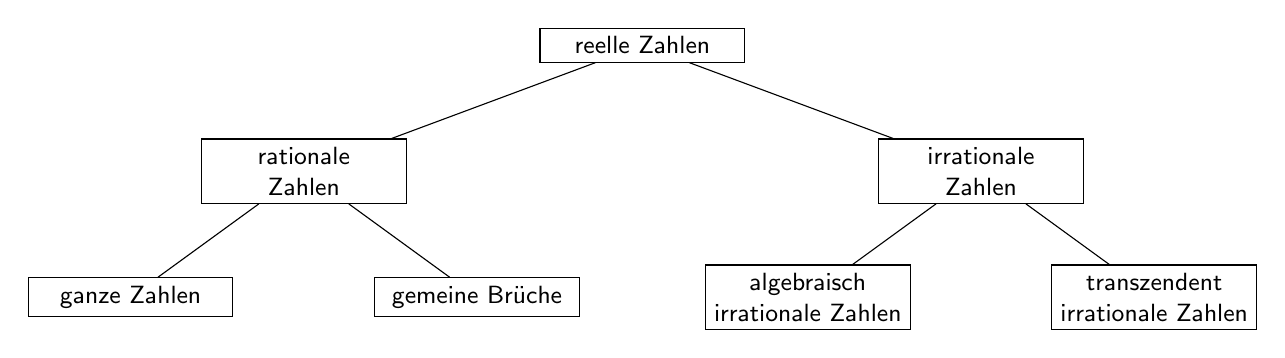
\begin{tikzpicture}[
      box/.style={draw, rectangle, align=center, font=\sffamily\small, inner sep=3pt, minimum width=2.6cm},
      level distance=1.6cm,
      level 1/.style={sibling distance=8.6cm},
      level 2/.style={sibling distance=4.4cm}]
    \node[box] (r) {reelle Zahlen}
      child {node[box] (q) {rationale\\Zahlen}
        child {node[box] {ganze Zahlen}}
        child {node[box] {gemeine Brüche}}
      }
      child {node[box] (i) {irrationale\\Zahlen}
        child {node[box] {algebraisch\\irrationale Zahlen}}
        child {node[box] {transzendent\\irrationale Zahlen}}
      };
  \end{tikzpicture}
\end{center}

\subsection{Intervalle reeller Zahlen}

Teilmengen der Menge $\mathbb{R}$ der reellen Zahlen, die auf der Zahlengeraden durch zwei Randpunkte $a$ und $b$ mit $a \leq b$ begrenzt werden, heißen \textbf{Intervalle}. Man unterscheidet endliche Intervalle und unendliche Intervalle.

Für \textbf{endliche Intervalle} gilt die folgende Nomenklatur:
\begin{itemize}
  \item offenes Intervall: alle $x$ mit $a < x < b$.\\
  Schreibweise: $I = (a,b)$
  \item rechtsseitig halboffenes Intervall: alle $x$ mit $a \leq x < b$.\\
  Schreibweise: $I = [a,b)$
  \item linksseitig halboffenes Intervall: alle $x$ mit $a < x \leq b$.\\
  Schreibweise: $I = (a,b]$
  \item abgeschlossenes Intervall: alle $x$ mit $a \leq x \leq b$.\\
  Schreibweise: $I = [a,b]$
\end{itemize}

Für \textbf{unendliche Intervalle} gilt:
\begin{itemize}
  \item $a \leq x \leq \infty$: $I = [a,\infty)$
  \item $a < x < \infty$: $I = (a,\infty)$
  \item $-\infty < x \leq b$: $I = (-\infty,b]$
  \item $-\infty < x < b$: $I = (-\infty,b)$
  \item $-\infty < x < +\infty$: $I = (-\infty,+\infty)$
\end{itemize}

Hinweis: Das offene Intervall $(a,b)$ wird gelegentlich auch durch die Schreibweise $]a,b[$ gekennzeichnet.

Intervalle kann man sich als »zusammenhängende Stücke« auf der reellen Zahlengeraden vorstellen. Die Eigenschaften »offen« und »abgeschlossen« zeigen dabei an, ob die jeweiligen Randpunkte dazugehören oder nicht. Selbstverständlich gibt es auch Mengen reeller Zahlen, die keine Intervalle sind, in Anwendungen hat man es allerdings sehr oft mit Intervallen zu tun. Beispiel ist eine Fragestellung der Art: Für welche möglichen Verkaufspreise eines bestimmten Produkts wird ein Gewinn erwirtschaftet? Hier wird in der Regel die Antwort nicht ein einziger Preis sein, sondern eine Palette möglicher Preise -- eben ein Intervall.

\subsubsection{Beispiele}

\begin{enumerate}[label=\alph*)]
  \item Alle reellen Zahlen $x$ mit $x \geq 1$ und $x \leq 4$ bilden ein Intervall, nämlich $[1,4]$.
  \item Die reellen Zahlen $x$, für die gilt $x \leq 1$ oder $x \geq 4$, bilden kein Intervall.\beispielende
\end{enumerate}

Interessant ist nun, was aus Intervallen wird, wenn man auf sie die üblichen Mengenoperationen Durchschnitt, Vereinigung und Komplementbildung anwendet. Man überzeugt sich zum Beispiel leicht davon (am besten mit Hilfe der Zahlengeraden!), dass der Durchschnitt $[-5,3] \cap [0,6]$ gleich dem Intervall $[0,3]$ ist. Für die Vereinigung gilt: $[-5,3] \cup [0,6] = [-5,6]$.

Ein Intervall reeller Zahlen enthält, sofern es nicht leer ist oder nur aus einem Element besteht, immer unendlich viele reelle Zahlen. Allgemein kann eine Teilmenge reeller Zahlen natürlich auch aus nur endlich vielen Elementen bestehen. Auf solche Mengen trifft man beispielsweise beim \textbf{Lösen von Gleichungen}. Man betrachte etwa die Gleichung
\[ x^2 + x - 5 = 1 . \]
Eine reelle Zahl, die für $x$ eingesetzt zu einer richtigen Aussage führt, nennt man \textbf{Lösung} dieser Gleichung. Wie manche Leser vielleicht inzwischen schnell errechnet haben, gibt es die zwei Lösungen $x = 2$ und $x = -3$. Man sagt nun auch, die obige Gleichung habe die \textbf{Lösungsmenge} $L = \{2,-3\}$.

Auf die Lösungsmengen von Gleichungen kommen wir noch zurück.

\structhead{Von der Zahlengeraden zur Ebene}

Zum Abschluss wollen wir von der \textbf{Zahlengeraden} zur \textbf{Ebene} übergehen.

In einem sogenannten \textbf{kartesischen Koordinatensystem} lässt sich die Lage eines Punktes $P$ in der Ebene durch zwei Zahlen beschreiben. Das kartesische Koordinatensystem besteht aus zwei senkrecht aufeinander stehenden Geraden, die waagerechte Gerade wird $x$-Achse oder \textbf{Abszisse} genannt, die dazu senkrechte Gerade heißt $y$-Achse oder \textbf{Ordinate}.

\subsubsection{Beispiel}

Hier sind zwei Punkte eingezeichnet:

\begin{center}
  \begin{tikzpicture}[scale=0.9]
    \draw[-{Stealth}] (-1.6,0) -- (4.2,0) node[below] {$x$};
    \draw[-{Stealth}] (0,-1.4) -- (0,3.8) node[left] {$y$};
    \foreach \x in {-1,1,2,3} { \draw (\x,-0.1) -- (\x,0.1); \node[below] at (\x,-0.1) {\x}; }
    \foreach \y in {-1,1,2,3} { \draw (-0.1,\y) -- (0.1,\y); \node[left] at (-0.1,\y) {\y}; }
    \draw[dotted] (2,0) -- (2,3) -- (0,3);
    \draw[dotted] (3,0) -- (3,2) -- (0,2);
    \fill (2,3) circle (2pt) node[above right] {$P_2(2,3)$};
    \fill (3,2) circle (2pt) node[above right] {$P_1(3,2)$};
  \end{tikzpicture}
\end{center}

Der Abstand von $P_1$ zur $y$-Achse ist $x_1 = 3$. Der Abstand von $P_1$ zur $x$-Achse ist $y_1 = 2$. Das Zahlenpaar $(x_1;y_1)$ beschreibt den Punkt $P_1$:
\[ P_1 = (x_1;y_1) = (3;2) \]
Die beiden Koordinaten $x_1$ und $y_1$ dürfen nicht vertauscht werden, wenn der Punkt $P_1$ durch sie beschrieben werden soll. Durch Vertauschung der beiden Koordinaten erhält man den Punkt $P_2 = (x_2;y_2) = (2;3)$. $P_1 = (3;2)$ und $P_2 = (2;3)$ sind verschiedene Punkte. Sie werden jeweils durch ein \textbf{geordnetes Paar} von Zahlen beschrieben.\definitionsende

Zwei geordnete Paare $(x_1;y_1)$ und $(x_2;y_2)$ sind nur dann gleich, wenn $x_1 = x_2$ und $y_1 = y_2$ ist. Wir schreiben dann auch $(x_1;y_1) = (x_2;y_2)$.

Zusammenfassend sagen wir noch einmal: Die Menge $\mathbb{R}$ aller reellen Zahlen kann geometrisch durch die Menge aller Punkte der Zahlengeraden dargestellt werden. Die Menge aller reellen Zahlenpaare $(x;y)$ wird geometrisch durch die Menge aller Punkte der Ebene repräsentiert.

\subsection{Übungsaufgaben zu Abschnitt 1.2}

\begin{uebungsaufgaben}
  \item Geben Sie jeweils an, zu welcher der Mengen $\mathbb{N}$, $\mathbb{Z}$, $\mathbb{Q}$ oder $\mathbb{R}$ die folgenden Zahlen gehören:
    \begin{enumerate}[label=\alph*)]
      \item $\dfrac{45}{13}$
      \item $2{,}38$
      \item $1024$
      \item $e^2$
    \end{enumerate}
  \item Stellen Sie folgende Zahlen, falls möglich, jeweils als Bruch dar:
    \begin{enumerate}[label=\alph*)]
      \item $1{,}5$
      \item $\sqrt{3}$
      \item $3{,}\overline{14}$
      \item $\dfrac{\pi}{2}$
    \end{enumerate}
  \item Schreiben Sie die folgenden Mengen als Intervalle:
    \begin{enumerate}[label=\alph*)]
      \item $\{x \in \mathbb{R} \mid x < 7\}$
      \item $\{a \in \mathbb{R} \mid 7 < a < 9\}$
      \item $\{y \in \mathbb{R} \mid y \leq 4\}$
      \item $\{z \in \mathbb{R} \mid 3 \leq z \leq 9\}$
    \end{enumerate}
  \item Schreiben Sie die folgenden Intervalle als Mengen:
    \begin{enumerate}[label=\alph*)]
      \item $[12,985]$
      \item $[4,\infty)$
      \item $(-\infty,-4)$
    \end{enumerate}
  \item Man untersuche, ob die folgenden Mengen Intervalle sind:
    \begin{enumerate}[label=\alph*)]
      \item $[1,2] \cap [2,3]$
      \item $[1,2] \cup [2,3]$
      \item $[1,2] \cup [3,4]$
      \item $\overline{[1,2]}_{\mathbb{R}}$
      \item $\overline{(-\infty,2)}_{\mathbb{R}}$
    \end{enumerate}
  \item Überlegen Sie, unter welchen Bedingungen die Vereinigung zweier Intervalle wieder ein Intervall ist.
  \item Tragen Sie die drei Punkte $(-1;-1)$, $(\tfrac{1}{2};2)$ und $(2;5)$ in ein kartesisches Koordinatensystem ein. Was fällt Ihnen auf?
\end{uebungsaufgaben}

\subsection{Lösungen der Übungsaufgaben zu 1.2}

\loesung{1.2.7.1:}
Alle Zahlen sind reell und somit in $\mathbb{R}$. Weiter gilt:
\begin{enumerate}[label=\alph*)]
  \item $\tfrac{45}{13}$ ist Element von $\mathbb{Q}$, jedoch nicht von $\mathbb{Z}$ oder $\mathbb{N}$.
  \item wie a).
  \item Es gilt $1024 \in \mathbb{N}$ und damit natürlich auch $1024 \in \mathbb{Z}$, $1024 \in \mathbb{Q}$ und $1024 \in \mathbb{R}$.
  \item $e^2$ ist irrational und somit weder in $\mathbb{Q}$ noch in $\mathbb{Z}$ oder $\mathbb{N}$.
\end{enumerate}

\loesung{1.2.7.2:}
\begin{enumerate}[label=\alph*)]
  \item $1{,}5 = \tfrac{3}{2}$
  \item $\sqrt{3}$ ist kein Bruch, d.\,h. $\sqrt{3} \notin \mathbb{Q}$.
  \item $3{,}\overline{14} = 3 + \tfrac{14}{99} = \tfrac{311}{99}$
  \item $\tfrac{\pi}{2} \notin \mathbb{Q}$.
\end{enumerate}

\loesung{1.2.7.3:}
\begin{enumerate}[label=\alph*)]
  \item $(-\infty,7)$
  \item $(7,9)$
  \item $(-\infty,4]$
  \item $[3,9]$
\end{enumerate}

\loesung{1.2.7.4:}
\begin{enumerate}[label=\alph*)]
  \item $\{x \in \mathbb{R} \mid 12 \leq x \leq 985\}$
  \item $\{y \in \mathbb{R} \mid y \geq 4\}$
  \item $\{z \in \mathbb{R} \mid z < -4\}$
\end{enumerate}

\loesung{1.2.7.5:}
\begin{enumerate}[label=\alph*)]
  \item $[1,2] \cap [2,3] = \{2\} = [2,2]$ ist Intervall.
  \item $[1,2] \cup [2,3] = [1,3]$ ist Intervall.
  \item $[1,2] \cup [3,4]$ ist kein Intervall.
  \item $\overline{[1,2]}_{\mathbb{R}}$ ist kein Intervall.
  \item $\overline{(-\infty,2)}_{\mathbb{R}} = [2,\infty)$ ist Intervall.
\end{enumerate}

\loesung{1.2.7.6:}
Die Vereinigung zweier Intervalle ist genau dann ein Intervall, wenn sie sich überschneiden oder nach Hinzunahme ihrer Endpunkte mindestens ein Element gemeinsam haben, welches schon zu einem der beiden Intervalle gehört.

\loesung{1.2.7.7:}
Die drei Punkte liegen auf einer Geraden.

\begin{center}
  \begin{tikzpicture}[scale=0.55]
    \draw[->] (-2.2,0) -- (6.2,0) node[below] {$x$};
    \draw[->] (0,-2.4) -- (0,6.4) node[left] {$y$};
    \foreach \x in {-1,1,2} { \draw (\x,-0.1) -- (\x,0.1) node[below] {\small\x}; }
    \foreach \y in {-2,...,6} { \draw (-0.1,\y) -- (0.1,\y) node[left] {\small\y}; }
    \draw[blue] (-2.0,-3.0) -- (2.5,6.0);
    \fill[blue] (-1,-1) circle (2pt);
    \fill[blue] (0.5,2) circle (2pt);
    \fill[blue] (2,5) circle (2pt);
  \end{tikzpicture}
\end{center}
